\documentclass{article}
\pagestyle{empty}

\usepackage[normalem]{ulem}

% set up page size and margins
%\usepackage[letterpaper,landscape,centering,margin=0.5in]{geometry}
%\usepackage[screen,centering,margin=0.5in]{geometry}
\usepackage[paperwidth=240mm,paperheight=180mm,centering,margin=0.5in]{geometry}

% this was recommended by psnfss2e.pdf
%\usepackage{textcomp}
%\usepackage{txfonts}
%\renewcommand{\rmdefault}{cm}
%\usepackage{lmodern}
%\usepackage[Symbol]{upgreek}
%\newcommand{\alphaup}{\upalpha}
%%% Upright Greek letters
\usepackage{amsfonts}
\DeclareSymbolFont{UPM}{U}{eur}{m}{n}
\SetSymbolFont{UPM}{bold}{U}{eur}{b}{n}
\DeclareMathSymbol{\upalpha}{0}{UPM}{"0B}
\DeclareMathSymbol{\upbeta}{0}{UPM}{"0C}
%\usepackage[math]{kurier}
%\renewcommand{\rmdefault}{cm}
\usepackage[T1]{fontenc}
\usepackage{cmbright}
%\usepackage{ccfonts}

%\usepackage{psfonts}

%\usepackage{helvet}
%\usepackage{avant}

\usepackage{url}

%% % from http://www.superstrate.net/useful/useful.html
%% \DeclareFontFamily{U}{euc}{}% I chose euc because the chart is called Euler cursive
%% \DeclareFontShape{U}{euc}{m}{n}{<-6>eurm5<6-8>eurm7<8->eurm10}{}%
%% \DeclareSymbolFont{AMSc}{U}{euc}{m}{n} % I chose AMSc because AMSa and AMSb are defined in the amsfonts-package
%% \DeclareMathSymbol{\alphaup}{\mathord}{AMSc}{11}

% scale up the fonts and space things correctly


%\linespread{2}

%% stolen from file `a0poster.cls', modified by RHK shifted font sizes
%% down three lines (and added three smaller sizes)
\renewcommand{\tiny}        {\fontsize{6.95}{8.68}\selectfont}    
\renewcommand{\scriptsize}  {\fontsize{8.33}{10.42}\selectfont}    
\renewcommand{\footnotesize}{\fontsize{10}{12.5}\selectfont}    
\renewcommand{\small}       {\fontsize{12}{14}\selectfont}    
\renewcommand{\normalsize}  {\fontsize{14.4}{18}\selectfont}  
\renewcommand{\large}       {\fontsize{17.28}{22}\selectfont} 
\renewcommand{\Large}       {\fontsize{20.74}{25}\selectfont} 
\renewcommand{\LARGE}       {\fontsize{24.88}{30}\selectfont} 
\renewcommand{\huge}        {\fontsize{26.5}{32}\selectfont} 
\renewcommand{\Huge}        {\fontsize{35.83}{45}\selectfont} 
\newcommand{\veryHuge}      {\fontsize{43}{54}\selectfont}    
\newcommand{\VeryHuge}      {\fontsize{51.6}{64}\selectfont}  
\newcommand{\VERYHuge}      {\fontsize{61.92}{77}\selectfont} 
%			    {\fontsize{74.3}{93}\selectfont}  
%			    {\fontsize{89.16}{112}\selectfont}
%			    {\fontsize{107}{134}\selectfont}  

% These colours are tried and tested for titles and headers. Don't
% over use color!
\usepackage{color}
\definecolor{DarkBlue}{rgb}{0.1,0.1,0.5}
\definecolor{Red}{rgb}{0.8,0.0,0.0}
\definecolor{Purple}{rgb}{0.8,0.0,0.8}
\definecolor{LightRed}{rgb}{1.0,0.0,0.0}
\definecolor{Cyan}{rgb}{0.0,0.9,0.9}
\definecolor{Magenta}{rgb}{0.9,0.0,0.9}
\definecolor{Green}{rgb}{0.0,0.9,0.0}
\definecolor{PicBlue}{rgb}{0.098,0.082,0.227}

%% stolen from http://www.edwardtufte.com/tufte/
\definecolor{ETYellow}{rgb}{1,1,0.953}

%% I've made it darker to calm the effect when projected on a large
%% screen
\definecolor{BGYellow}{rgb}{0.95,0.95,0.85}
% \definecolor{BGYellow}{rgb}{0.9,0.9,0.7}
%\pagecolor{BGYellow}

% see documentation for a0poster class for the size options here
\def\Head#1{\noindent\begin{center}{\Large\color{DarkBlue}#1}\end{center}}
\def\Important#1{\noindent{\color{Red} #1}}
\def\ImportantB#1{\noindent{ #1}}
\def\LHead#1{\noindent{\Large #1}}
\def\Title#1{\noindent\begin{center}{\Huge\color{Red}#1}\end{center}}
\def\Subtitle#1{\noindent\begin{center}{\huge\color{DarkBlue}#1}\end{center}}

% select the right font
%\renewcommand{\familydefault}{\sfdefault}

% The textpos package is necessary to position textblocks at arbitary 
% places on the page.
\usepackage[absolute,overlay]{textpos}

\usepackage{amsmath}
\usepackage{amssymb}

% Graphics to include graphics. Times is nice on posters, but you
% might want to switch it off and go for CMR fonts.
%\usepackage{graphics,wrapfig,times}
\usepackage{graphicx,wrapfig}

\TPGrid[0.5in,0.5in]{10}{10} % 2 cols of width 4.5, plus 1 gap of width 1

\parindent=0pt
\parskip=0.5\baselineskip

\begin{document}
\large

\pagecolor{white}

\begin{textblock}{10}(-1,-3)\Large\centering
\includegraphics[width=12\TPHorizModule]{images/M87.jpg}
\end{textblock}

\begin{textblock}{10}(0,3)
\Title{\textcolor{white}{\textbf{Uncertainty versus Decisions}}}
\Subtitle{\textcolor{Cyan}{Some (false) dichotomies between\\ Astrophysics and Machine Learning}}
\end{textblock}

\begin{textblock}{10}(0,0.2)
\large \textcolor{Cyan}{Roban Hultman Kramer}
\end{textblock}

\begin{textblock}{3}(7,0)
\includegraphics[width=3\TPHorizModule]{images/ht-logo.png}
\end{textblock}

\begin{textblock}{10}(0,10)\centering
\small
\texttt{robanhk@gmail.com} \hspace{1in} \texttt{http://roban.github.com}
\end{textblock}

%%%%%%%%%%%%%%%%%%%%%%%%%%%%%%%%%%%%%%%%%%%%%%%%%%%%%%%%%%%%%%%%%%%%%%%%%%%%%%
\
\clearpage
%%%%%%%%%%%%%%%%%%%%%%%%%%%%%%%%%%%%%%%%%%%%%%%%%%%%%%%%%%%%%%%%%%%%%%%%%%%%%%

\pagecolor{white}
\begin{textblock}{5}(0,0)
\centering {\huge Astrophysics}
\end{textblock}

\begin{textblock}{5}(5,0)
\centering {\huge Machine Learning}
\end{textblock}

\begin{textblock}{5}(0,2)\Large
\centering \textcolor{Red}{\veryHuge Uncertainty \\ is \\ everything\\}

\vspace{1in}

Constraining Parameters  \vspace{0.5in} \\
\end{textblock}

\begin{textblock}{1}(4.5,0.75)
\centering {\Huge vs.\vspace{1in}}
\end{textblock}

\begin{textblock}{5}(5,2)\Large
\centering \textcolor{DarkBlue}{\veryHuge Decisions \\ are \\ everything\\}

\vspace{1in}

Making Predictions  \vspace{0.5in} \\

\end{textblock}


%%%%%%%%%%%%%%%%%%%%%%%%%%%%%%%%%%%%%%%%%%%%%%%%%%%%%%%%%%%%%%%%%%%%%%%%%%%%%%
\
\clearpage
%%%%%%%%%%%%%%%%%%%%%%%%%%%%%%%%%%%%%%%%%%%%%%%%%%%%%%%%%%%%%%%%%%%%%%%%%%%%%%

\pagecolor{white}
\begin{textblock}{5}(0,0)
\centering {\huge Astrophysics}
\end{textblock}

\begin{textblock}{10}(1.2,1.2)\Large
\includegraphics[width=8\TPHorizModule]{images/qso_spectrum.pdf}\\
\end{textblock}

\begin{textblock}{10}(0,9.7)\Large\centering
The uncertainty of the measurement is as important as the value.
\end{textblock}

\begin{textblock}{10}(1.5,0.7)\Large
\textcolor{Red}{\veryHuge Uncertainty is everything}\\
\end{textblock}


%%%%%%%%%%%%%%%%%%%%%%%%%%%%%%%%%%%%%%%%%%%%%%%%%%%%%%%%%%%%%%%%%%%%%%%%%%%%%%
\
\clearpage
%%%%%%%%%%%%%%%%%%%%%%%%%%%%%%%%%%%%%%%%%%%%%%%%%%%%%%%%%%%%%%%%%%%%%%%%%%%%%%

\pagecolor{white}
\begin{textblock}{5}(0,0)
\centering {\huge Astrophysics}
\end{textblock}

\begin{textblock}{10}(-1,1.3)\Large\centering
\includegraphics[height=8\TPVertModule]{images/qso_spectrum_posterior.pdf}\\
\end{textblock}

\begin{textblock}{10}(0,9.7)\Large\centering
The uncertainty of the parameter is as important as the value.
\end{textblock}

\begin{textblock}{10}(1.5,0.7)\Large
\textcolor{Red}{\veryHuge Uncertainty is everything}

posterior distribution of parameters from MCMC
\end{textblock}


%%%%%%%%%%%%%%%%%%%%%%%%%%%%%%%%%%%%%%%%%%%%%%%%%%%%%%%%%%%%%%%%%%%%%%%%%%%%%%
\
\clearpage
%%%%%%%%%%%%%%%%%%%%%%%%%%%%%%%%%%%%%%%%%%%%%%%%%%%%%%%%%%%%%%%%%%%%%%%%%%%%%%

\pagecolor{white}
\begin{textblock}{5}(0,0)
\centering {\huge Astrophysics}
\end{textblock}

\begin{textblock}{10}(7.5,-0.5)
\includegraphics[height=4\TPVertModule]{images/qso_spectrum_posterior.pdf}\\
\end{textblock}

\begin{textblock}{8}(1,4)\Large
\includegraphics[height=4\TPVertModule]{images/plate.pdf}\\
\end{textblock}

\begin{textblock}{6}(5,4)
Population level:\\
distribution of parameter vectors

$p(\theta_i| \mu, \sigma) \sim N(\mu, \sigma)$
\vspace{0.5in}

Quasar level:\\
likelihood of observed spectrum\\given model

$p(F_{i,j} | \theta_i) \sim \cdots$

\end{textblock}

\begin{textblock}{10}(0,9.7)\Large\centering

\end{textblock}

\begin{textblock}{10}(1.5,0.7)\Large
\textcolor{Red}{\veryHuge Uncertainty is everything}\\
hierarchical model of the population\\ and individual objects
\end{textblock}

%%%%%%%%%%%%%%%%%%%%%%%%%%%%%%%%%%%%%%%%%%%%%%%%%%%%%%%%%%%%%%%%%%%%%%%%%%%%%%
\
\clearpage
%%%%%%%%%%%%%%%%%%%%%%%%%%%%%%%%%%%%%%%%%%%%%%%%%%%%%%%%%%%%%%%%%%%%%%%%%%%%%%

\pagecolor{white}
\begin{textblock}{5}(0,0)
\centering {\huge Astrophysics}
\end{textblock}

\begin{textblock}{10}(7.5,-0.5)
\includegraphics[height=4\TPVertModule]{images/qso_spectrum_posterior.pdf}\\
\end{textblock}

\begin{textblock}{10}(7.5,4)
\includegraphics[height=4\TPVertModule]{images/plate.pdf}\\
\end{textblock}

\begin{textblock}{10}(-1,1.3)\Large\centering
\includegraphics[height=8\TPVertModule]{images/Lya_CIV_peak_cor.png}\\
\end{textblock}


\begin{textblock}{10}(0,9.7)\Large\centering
hierarchical model of the population and individual objects
\end{textblock}

\begin{textblock}{10}(1.5,0.7)\Large
\textcolor{Red}{\veryHuge Uncertainty is everything}

distribution of the population
\end{textblock}



%%%%%%%%%%%%%%%%%%%%%%%%%%%%%%%%%%%%%%%%%%%%%%%%%%%%%%%%%%%%%%%%%%%%%%%%%%%%%%
\
\clearpage
%%%%%%%%%%%%%%%%%%%%%%%%%%%%%%%%%%%%%%%%%%%%%%%%%%%%%%%%%%%%%%%%%%%%%%%%%%%%%


\pagecolor{white}
\begin{textblock}{5}(0,0)
\centering {\huge Astrophysics}
\end{textblock}

\begin{textblock}{5}(5,0)
\centering {\huge Machine Learning}
\end{textblock}

\begin{textblock}{5}(0,1)\Large
\centering \textcolor{Red}{\VERYHuge Uncertainty} \vspace{0.1in}

\textcolor{Red}{\huge Example: MCMC}  \vspace{0.1in} \\
exploring parameter space\\
\includegraphics[width=4\TPHorizModule]{images/MCMC.pdf}
\end{textblock}

\begin{textblock}{1}(4.5,0.75)
\centering {\VERYHuge vs.\vspace{1in}}
\end{textblock}

\begin{textblock}{5}(5,1)\Large
\centering \textcolor{DarkBlue}{\VERYHuge Decisions}  \vspace{0.1in}

\textcolor{DarkBlue}{\huge Example: SVM}  \vspace{0.1in} \\
finding boundaries in feature space\\
\includegraphics[width=4\TPHorizModule]{images/445px-Svm_max_sep_hyperplane_with_margin.png}

\tiny Credit: Wikimedia Commons\\ \texttt{http://en.wikipedia.org/wiki/File:Svm\_max\_sep\_hyperplane\_with\_margin.png}
\end{textblock}


%%%%%%%%%%%%%%%%%%%%%%%%%%%%%%%%%%%%%%%%%%%%%%%%%%%%%%%%%%%%%%%%%%%%%%%%%%%%%%
\
\clearpage
%%%%%%%%%%%%%%%%%%%%%%%%%%%%%%%%%%%%%%%%%%%%%%%%%%%%%%%%%%%%%%%%%%%%%%%%%%%%%

\begin{textblock}{5}(5,0)
\centering {\huge Machine Learning}
\end{textblock}

\begin{textblock}{3}(0,0)
\includegraphics[width=3\TPHorizModule]{images/ht-logo.png}
\end{textblock}

\begin{textblock}{8}(1,0.7)\Large
\hfill \textcolor{DarkBlue}{\VERYHuge Decisions are everything}
\end{textblock}

\begin{textblock}{5}(0.5,2.0)\Large
\textbf{Problems:}\\
tagging of incoming content\\
classification of new users\\
\vspace{0.5in}
\end{textblock}

\begin{textblock}{5}(5.0,2.0)\Large
\textbf{Challenges:}\\
free-text tags are not consistent\\
\end{textblock}

\begin{textblock}{10}(0.0,3.5)\Large\centering
\includegraphics[width=6\TPHorizModule]{images/labels_discussions_dochist.png}

\textit{when humans tag}
\end{textblock}

%%%%%%%%%%%%%%%%%%%%%%%%%%%%%%%%%%%%%%%%%%%%%%%%%%%%%%%%%%%%%%%%%%%%%%%%%%%%%%
\
\clearpage
%%%%%%%%%%%%%%%%%%%%%%%%%%%%%%%%%%%%%%%%%%%%%%%%%%%%%%%%%%%%%%%%%%%%%%%%%%%%%

\begin{textblock}{5}(5,0)
\centering {\huge Machine Learning}
\end{textblock}

\begin{textblock}{3}(0,0)
\includegraphics[width=3\TPHorizModule]{images/ht-logo.png}
\end{textblock}

\begin{textblock}{8}(1,0.7)\Large
\hfill \textcolor{DarkBlue}{\VERYHuge Decisions are everything}
\end{textblock}

\begin{textblock}{5}(0.5,2.0)\Large
\textbf{Problems:}\\
tagging of incoming content\\
classification of new users\\
\vspace{0.5in}
\end{textblock}

\begin{textblock}{5}(5.0,2.0)\Large
\textbf{Challenges:}\\
free-text tags are not consistent\\
\end{textblock}

\begin{textblock}{8}(1.,4.0)
\textbf{Potential Solutions:}\\
\textbf{fully-automatic tags?} -- not accurate enough, want human
validation\\
\textbf{pre-defined categories?} -- feels limiting and arduous
\end{textblock}


%%%%%%%%%%%%%%%%%%%%%%%%%%%%%%%%%%%%%%%%%%%%%%%%%%%%%%%%%%%%%%%%%%%%%%%%%%%%%%
\
\clearpage
%%%%%%%%%%%%%%%%%%%%%%%%%%%%%%%%%%%%%%%%%%%%%%%%%%%%%%%%%%%%%%%%%%%%%%%%%%%%%

\begin{textblock}{5}(5,0)
\centering {\huge Machine Learning}
\end{textblock}

\begin{textblock}{3}(0,0)
\includegraphics[width=3\TPHorizModule]{images/ht-logo.png}
\end{textblock}

\begin{textblock}{8}(1,0.7)\Large
\hfill \textcolor{DarkBlue}{\VERYHuge Decisions are everything}
\end{textblock}

\begin{textblock}{5}(0.5,2.0)\Large
\textbf{Problems:}\\
tagging of incoming content\\
classification of new users\\
\vspace{0.5in}
\end{textblock}

\begin{textblock}{5}(5.0,2.0)\Large
\textbf{Challenges:}\\
free-text tags are not consistent\\
\end{textblock}

\begin{textblock}{8}(1.,4.0)
\textbf{Potential Solutions:}\\
\textbf{fully-automatic tags?} -- not accurate enough, want human
validation\\
\textbf{pre-defined categories?} -- feels limiting and arduous
\vspace{0.5in}

\textbf{Implemented Solution:}\\
train classifiers (e.g. SVM, logistic regression) on best tags\\
suggest high-confidence tags to users for validation\\
\vspace{0.1in}

\textit{Forces a decision:} show a tag or don't.
\end{textblock}

%%%%%%%%%%%%%%%%%%%%%%%%%%%%%%%%%%%%%%%%%%%%%%%%%%%%%%%%%%%%%%%%%%%%%%%%%%%%%%
\
\clearpage
%%%%%%%%%%%%%%%%%%%%%%%%%%%%%%%%%%%%%%%%%%%%%%%%%%%%%%%%%%%%%%%%%%%%%%%%%%%%%


\pagecolor{white}
\begin{textblock}{5}(0,0)
\centering {\huge Astrophysics}
\end{textblock}

\begin{textblock}{5}(5,0)
\centering {\huge Machine Learning}
\end{textblock}

\begin{textblock}{5}(0,1)\Large
\centering \textcolor{Red}{\VERYHuge \sout{Uncertainty}}
\end{textblock}

\begin{textblock}{5}(5,1)\Large
\centering \textcolor{DarkBlue}{\VERYHuge Decisions}  \vspace{0.1in}
\end{textblock}


\begin{textblock}{1}(4.5,0.75)
\centering {\VERYHuge vs.\vspace{1in}}\vspace{0.1in}
\end{textblock}

\begin{textblock}{5}(0,2)\Large\centering
{\Huge Counter Example}\vspace{0.1in}

\centering \textcolor{Red}{\VERYHuge Decisions} \vspace{0.1in}

planning observations\\
target selection\vspace{0.2in}

\textbf{Limited by:}\\
telescope time\\
instrument budgets

(Hubble oversubscribed by $\approx 600\%$)

\end{textblock}

\begin{textblock}{5}(5,4.1)\Large\centering
recommendation engines\\
targeted marketing\vspace{0.2in}

\textbf{Limited by:}\\
user attention span\\
marketing budgets
\end{textblock}

%%%%%%%%%%%%%%%%%%%%%%%%%%%%%%%%%%%%%%%%%%%%%%%%%%%%%%%%%%%%%%%%%%%%%%%%%%%%%%
\
\clearpage
%%%%%%%%%%%%%%%%%%%%%%%%%%%%%%%%%%%%%%%%%%%%%%%%%%%%%%%%%%%%%%%%%%%%%%%%%%%%%


\pagecolor{white}
\begin{textblock}{5}(5,0)
\centering {\huge Machine Learning}
\end{textblock}

\begin{textblock}{5}(5,2)
\centering \textit{\LARGE evaluating results\vspace{1in}}
\end{textblock}

\begin{textblock}{5}(5,1)\Large
\centering \textcolor{DarkBlue}{\VERYHuge Decisions}  \vspace{0.75in}

$F_\beta$-scores\\
lift\\
ROC curves

\includegraphics[width=3.7\TPHorizModule]{images/Roccurves.png}

\tiny Wikimedia Commons \texttt{http://en.wikipedia.org/wiki/File:Roccurves.png}

\end{textblock}


%%%%%%%%%%%%%%%%%%%%%%%%%%%%%%%%%%%%%%%%%%%%%%%%%%%%%%%%%%%%%%%%%%%%%%%%%%%%%%
\
\clearpage
%%%%%%%%%%%%%%%%%%%%%%%%%%%%%%%%%%%%%%%%%%%%%%%%%%%%%%%%%%%%%%%%%%%%%%%%%%%%%


\pagecolor{white}
\begin{textblock}{5}(0,0)
\centering {\huge Astrophysics}
\end{textblock}

\begin{textblock}{5}(5,0)
\centering {\huge Machine Learning}
\end{textblock}

\begin{textblock}{5}(0,1)\Large
\centering \textcolor{Red}{\VERYHuge Uncertainty} \vspace{0.75in}

error bars\\
$p$-values\\
posterior distributions\\

\includegraphics[width=3.7\TPHorizModule]{images/posterior.pdf}
\end{textblock}

\begin{textblock}{1}(4.5,0.75)
\centering {\VERYHuge vs.\vspace{1in}}
\end{textblock}

\begin{textblock}{10}(0,2)
\centering \textit{\LARGE evaluating results\vspace{1in}}
\end{textblock}

\begin{textblock}{5}(5,1)\Large
\centering \textcolor{DarkBlue}{\VERYHuge Decisions}  \vspace{0.75in}

$F_\beta$-scores\\
lift\\
ROC curves

\includegraphics[width=3.7\TPHorizModule]{images/Roccurves.png}

\tiny Wikimedia Commons \texttt{http://en.wikipedia.org/wiki/File:Roccurves.png}

\end{textblock}

%%%%%%%%%%%%%%%%%%%%%%%%%%%%%%%%%%%%%%%%%%%%%%%%%%%%%%%%%%%%%%%%%%%%%%%%%%%%%%
\
\clearpage
%%%%%%%%%%%%%%%%%%%%%%%%%%%%%%%%%%%%%%%%%%%%%%%%%%%%%%%%%%%%%%%%%%%%%%%%%%%%%

\pagecolor{white}
\begin{textblock}{5}(0,0)
\centering {\huge Astrophysics}
\end{textblock}

\begin{textblock}{5}(5,0)
\centering {\huge Machine Learning}
\end{textblock}

\begin{textblock}{5}(0,1.1)\Large
\centering \textcolor{Red}{\textbf{Computational bottleneck:\\ model complexity}} \vspace{0.1in}
\end{textblock}

\begin{textblock}{5}(5,1.1)\Large
\centering \textcolor{DarkBlue}{\textbf{Computational bottleneck:\\ data size\vspace{0.5in}}}  \vspace{0.1in}
\end{textblock}


\begin{textblock}{1}(4.5,0.75)
\centering {\VERYHuge vs.\vspace{1in}}\vspace{0.1in}
\end{textblock}

\begin{textblock}{5}(0,3)\Large\centering
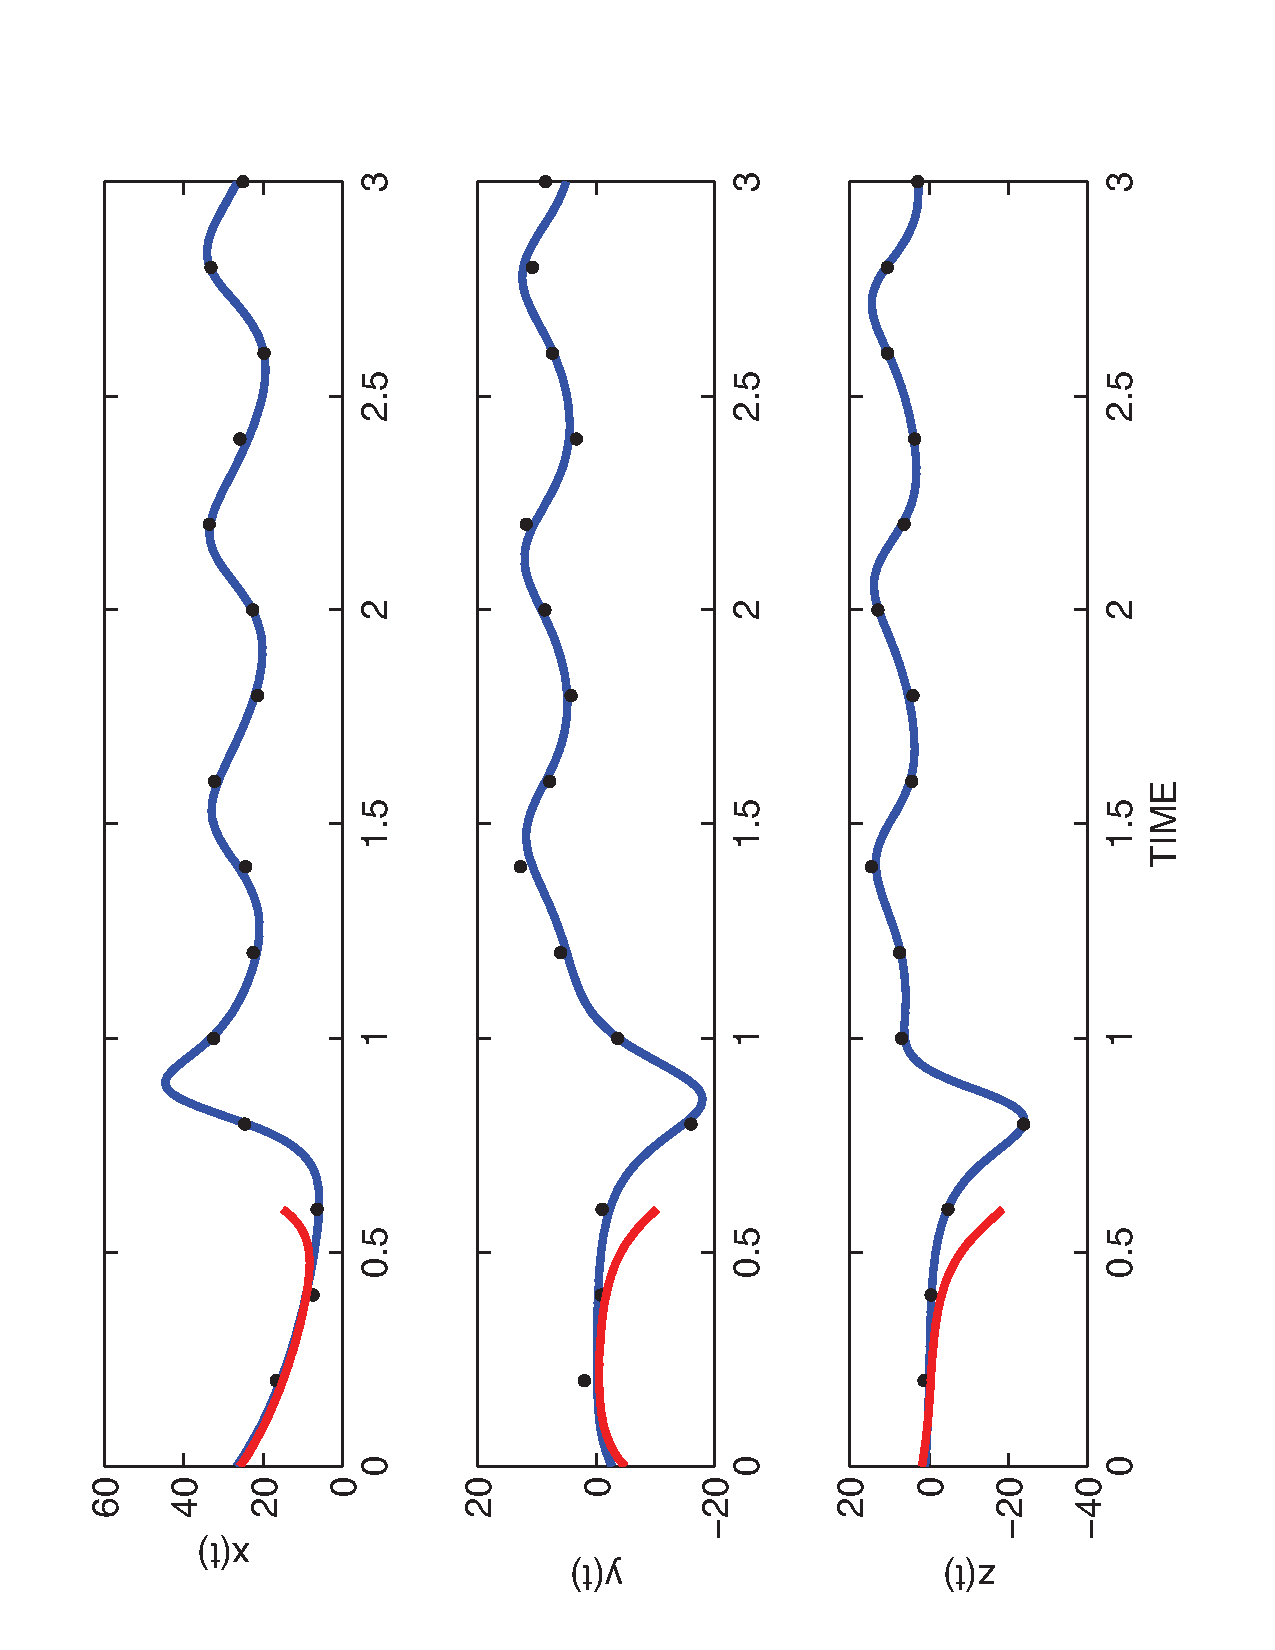
\includegraphics[height=5.0\TPHorizModule,
  angle=-90]{images/solonen_fig.pdf}

\tiny ``Efficient MCMC for Climate Model Parameter Estimation:
  Parallel Adaptive Chains and Early Rejection'' Solonen et al. \textit{Bayesian Analysis} 7, 3 (2012), 715-736.
\end{textblock}

\begin{textblock}{5}(5,3)\Large\centering
\includegraphics[width=5.0\TPHorizModule]{images/mantle-mahout.png}
\end{textblock}

%%%%%%%%%%%%%%%%%%%%%%%%%%%%%%%%%%%%%%%%%%%%%%%%%%%%%%%%%%%%%%%%%%%%%%%%%%%%%%
\
\clearpage
%%%%%%%%%%%%%%%%%%%%%%%%%%%%%%%%%%%%%%%%%%%%%%%%%%%%%%%%%%%%%%%%%%%%%%%%%%%%%

\begin{textblock}{5}(-1,-1)\Large\centering
\includegraphics[height=12\TPVertModule]{images/Dishes_overview_300dpi_white.jpg}
\end{textblock}

\pagecolor{white}
\begin{textblock}{5}(0,0)
\centering {\huge Astrophysics}
\end{textblock}

\begin{textblock}{5}(5,0)
\centering {\huge Machine Learning}
\end{textblock}

\begin{textblock}{5}(0,1.1)\Large
\centering \textcolor{Red}{\textbf{Computational bottleneck:\\ \sout{model complexity}}} \vspace{0.1in}
\end{textblock}

\begin{textblock}{5}(5,1.1)\Large
\centering \textcolor{DarkBlue}{\textbf{Computational bottleneck:\\ data size\vspace{0.5in}}}  \vspace{0.1in}
\end{textblock}


\begin{textblock}{1}(4.5,0.75)
\centering {\VERYHuge vs.\vspace{1in}}\vspace{0.1in}
\end{textblock}

\begin{textblock}{5}(0,3)\Large\centering
\bf\ 
{\Huge Counter Example}\vspace{0.1in}

\textcolor{Red}{The Square Kilometer Array}\\
Data Rate:\\ 1~TB \textbf{per second}\\
\textit{after} pre-processing\vspace{0.2in}


\textcolor{Red}{Computational bottleneck:\\ data size}
\end{textblock}

\begin{textblock}{10}(0,10.5)
{\small ``Artist's impression of the SKA dishes.'' Credit: SKA Organisation/TDP/DRAO/Swinburne Astronomy Productions}
\end{textblock}

%%%%%%%%%%%%%%%%%%%%%%%%%%%%%%%%%%%%%%%%%%%%%%%%%%%%%%%%%%%%%%%%%%%%%%%%%%%%%%
\
\clearpage
%%%%%%%%%%%%%%%%%%%%%%%%%%%%%%%%%%%%%%%%%%%%%%%%%%%%%%%%%%%%%%%%%%%%%%%%%%%%%



\end{document}
